\chapter{Prototype Implementation}

For the implementation of contracting service I have used Django framework because it is powerful but also easy to use because it provides a fixed structure to organize the project. Django framework provides built-in modules for most of the common functionalities with a good security architecture. Along with Django, I have used Bootstrap for styling because it is light-weight and simple.

In this chapter I will present a brief description of technologies that I used followed by a brief overview of the whole project, showing how different parts fit together before digging into details.

\section{Technologies Used}

\subsection{Django Framework}
\fixme{Mention which parts of django do I use, like login(authentication)/logout, admin page, etc}
\fixme{Also mention security measures like csrf protection and such}

\subsection{Bootstrap}
\fixme{Mention responsive}

\section{Overview}
\fixme{Mention how it all works (Admin, Manufacturer, Customer, User), CES+LWM2M, add picture from blackboard at end }

This solution is a Web platform for managing small devices and controlling who has access to the data they generate. Most challenging part was understanding the users of the platform and their needs. Following section describes account types which correspond to roles they have, followed by the brief description of main parts of the platform.

\subsection{Account Types}

In the Industrial Internet context I have identified four different types of accounts, with their separate views of the platform depending on their role. Views of these accounts have a common core although they are suited for different purposes. 

Firstly, there needs to be a central authority that distributes accounts to verified manufacturers of industrial machines. In order to receive manufacturer account you need to contact this central authority, which could be a standardization agency but it can be any impartial actor. When that authority verifies that your company is who they claim to be, several accounts can be issued depending on the number of departments that company has or any other criteria depending on the agreement with the manufacturer company. Since the only responsibility this authority have is creating accounts for manufacturers I have used standard Django admin page (and admin account) for its implementation, stripped down to only basic functionality for managing accounts.

Secondly, manufacturers account is assigned to companies that produce smart machines. Their responsibility is to add devices (and update their information if necessary) to platform and assign them to machines (detailed description of devices will be given in subsection ~\ref{deviceManagement}), which are abstract representation of real machine (such is a smart crane) and devices it possess. When the machine has been bought by the customer, manufacturer creates an account for customer (in case they do not possess one) and assigns it to them, giving them full control over who can communicate with that machine. Manufacturer account will be described in detail in section ~\ref{Manufacturer}.

Thirdly, customer account is assigned to owners of the smart machines. Their view is restricted to only devices and machines that they possess and they can manage policies (control access to devices) for those devices only. Along with the possibility of managing policies, customer account can create multiple user accounts (which represents people responsible for single machines or group of them) and assign machines or devices to them. In this way, customer account has a full overview of what policies are in place and who created them while also being able to add or remove faulty ones or general ones (like allowing his work computer to access all the data or opening their data to a statistical agency). By being able to create user accounts customer can \fixme{pass on} the responsibility and fine tuning of policies for certain machines down the hierarchy of the company.

Finally, user account is assigned to people responsible for a subset of machines that a customer company possess. These accounts are restricted to only managing policies of the machines assigned to them without the possibility to create more accounts or manage devices in the system. Overview of accounts and their views are visualized in figure ~\ref{fig:accountTypes}.

\begin{figure}[ht]
	\begin{center}
		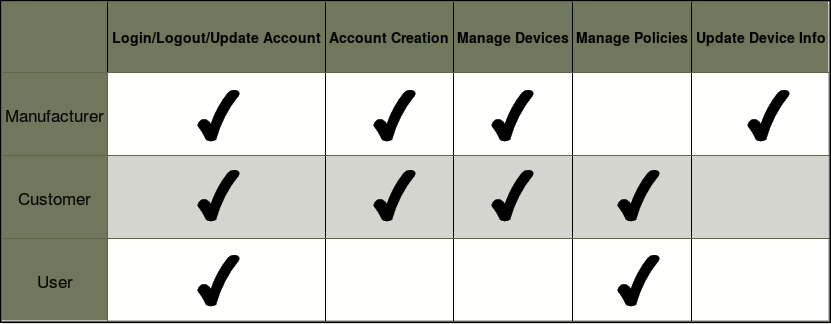
\includegraphics[width=\textwidth]{images/Functionalities}
		\caption{Account types and their views}
		\label{fig:accountTypes}
	\end{center}
\end{figure}

\subsection{Device Management}
\label{deviceManagement}

\subsection{Policy Management}
\label{policyManagement}

\section{Manufacturer}
\label{Manufacturer}

\section{Customer}

\section{User}
